% !TeX root = ../main.tex
\section{Results}
\label{sec:model_comparison}
%
The discretised-reflection model now allows us to revisit and extend established results on semiconductor lasers with FBG feedback. 
We first show that the EGM structure predicted by the model reproduces earlier findings from the literature with excellent agreement, while providing a more complete classification through analytic expressions and continuation methods. 
Building on this foundation, we then examine laser stability, demonstrating how reflection zeros interact with the laser centre frequency and relaxation oscillations in close parallel to previous studies, but on a far more concrete basis enabled by the present formulation.
%
%
\subsection{EGM Structure}
\label{subsec:EGM_structure}
%
\subsubsection{Comparison to multiple reflection FBG feedback}
\label{subsubsec:naumenko}
%
A considerably more elaborate treatment of FBG feedback was developed by Naumenko et al. \cite{naumenko2003characteristics,naumenko2004slow}, who modeled the feedback term $F(t)$ as the inverse Fourier transform of the product of the delayed electric field spectrum and the grating reflection spectrum $\rho(\w)$, see Appendix~\ref{app:EC_multiple}.
This formulation, summarised in the introduction, enabled them to capture the essential role of spectral filtering in reorganising EGMs by means of a Green-function formalism. 
Their model further incorporated nonlinear gain compression and thermally induced frequency chirp, which strongly affect stability under current modulation.
When these additional effects are neglected, and appropriate simplifications are made, their system reduces to the discretised-reflection formulation derived here (Appendix~\ref{app:multiple_EC_nondim}), with parameter set $(\a, P, T, \tau, C_p) = (4, 0.5, 123, 512, 0)$ and varying grating parameters $\eta$, $\wB$, and $\wz$.
%
\par
%
In their analysis, EGMs were constructed through a Green-function expansion rather than closed-form analytical conditions, leading to an involved but tractable calculation of mode frequencies.
As noted earlier, Naumenko \textit{et al.} identified the appearance of “satellite” EGM branches, separated from the central EGM ellipse by the reflection zeros of the FBG, as the bandwidth $\wz$ narrowed or detuning $\wB$ increased.
This insight was critical in establishing the connection between spectral features of the grating and the global organisation of EGMs, but the complexity of their feedback term limited the use of continuation methods and left the bifurcation structure only partially characterised.
%
\begin{figure}[!t]
    \centering

        \begin{overpic}[width=0.74\linewidth]{Images/rB_003_annotated.pdf}
            \put(-2,44){(b)}
            \put(-2,96){(a)}
        \end{overpic}\\
        \hspace{-2.2em}
        \begin{overpic}[width=0.65\linewidth]{Images/Naumenko_EGM_rB003.pdf}
            \put(-5,80){(c)}
        \end{overpic}

    \caption{Comparison of EGM structures from the multiple-reflection model of Naumenko \textit{et al.} and the discretised-reflection model. 
    Panel (a) shows the common FBG frequency responses corresponding to bandwidths with reflection zeros at $1/3$, $4/3$, and $20/3\,$GHz, giving nondimensionalised locations $\wz = 0.016\pi, \; 0.064\pi, \; 0.32\pi$. 
    A constant reflectivity $R=\sqrt{0.001}$ yields an effective feedback rate $\eta=0.085$. 
    Panels (b) and (c) plot the resulting EGMs for these bandwidths using the multiple-reflection formulation and the discretised model, respectively. 
    In both cases, EGM branches are distinguished by circles, diamonds, and squares, while the MGM is marked by $\times$.}
    
    \label{fig:Naumenko_rB003}
\end{figure}
%
\begin{figure}[!t]
    \centering

        \begin{overpic}[width=0.725\linewidth]{Images/rB_02_annotated.pdf}
            \put(-2,45){(b)}
            \put(-2,96){(a)}
        \end{overpic}\\
        \hspace{-0.3em}
        \begin{overpic}[width=0.612\linewidth]{Images/Naumenko_EGM_rB02.pdf}
            \put(-12,87){(c)}
        \end{overpic}

    \caption{Comparison of EGM structures for a detuned FBG under moderate feedback shown in (a) from the multiple-reflection model (b) and the discretised-reflection model (c) . 
    Here, a reflectivity $R=\sqrt{0.05}$ gives an effective feedback rate $\eta=0.600$, the first reflection zero at $10/3\,$GHz corresponds to $\wz=0.16\pi$, and a detuning of $8\,$GHz yields $\wB=0.384\pi$.}

    \label{fig:Naumenko_rB02}
\end{figure}
%
\par
%
Figure~\ref{fig:Naumenko_rB003} compares the EGM structures obtained from the multiple-reflection model of Naumenko \textit{et al.} \cite{naumenko2003characteristics} with those predicted by the discretised-reflection formulation for varying grating bandwidth. 
For the parameter set under consideration, the layer number $N=10$ was chosen, which exceeds the minimal value $N_\text{min}=7$ required for validity according to \eqref{eq:Nmin}. 
The solutions are plotted in the frequency–intensity plane ($I=|E|^2$), rather than the more common $(\w_s,N_s)$-projection, which results in an inversion of the cavity-mode structure about the frequency axis. 
Conversion of bandwidths from hertz to the nondimensionalised form $\wz$ was performed using the quoted photon lifetime $\tau_p=24$ ps \cite{naumenko2003characteristics}. 
%
\par
%
In the case of zero detuning and weak feedback (Figure~\ref{fig:Naumenko_rB003}), excellent agreement is achieved between the two models. 
For a wide Bragg-reflector bandwidth (here a main-lobe width of $40/3\,$GHz, corresponding to $2\wz=0.64\pi$ in nondimensional form), the EGMs trace a closed curve strongly resembling the ECM ellipse of the COF case. 
The maximal gain mode (MGM), marked by $\times$, is located near the edge of the left-hand side of this curve. 
Further information is provided in the discretised case, as the closed curve which traces the EGM solutions given by \eqref{eq:discretised_Ns_curve} is also shown in (c), giving a clearer picture of the seperate components.
As the FBG bandwidth narrows, the number of EGMs decreases and the EGM curve contracts, remaining confined within the main lobe of the reflection spectrum. 
This behaviour is fully consistent with the analytic results of Section~\ref{subsec:EGM_discretised} and with earlier studies of Lorentzian-filter feedback \cite{yousefi1999dynamical}. 
%
\par
%
For sufficiently narrow bandwidths, additional satellite EGMs appear, marked with triangles in Figure~\ref{fig:Naumenko_rB003}. 
These satellites arise from the side lobes of the FBG reflection spectrum and are a distinctive feature of grating-based feedback. 
Notably, they do not appear in the single Lorentzian-filter model under zero detuning, underscoring the richer spectral structure captured here. 
In this regime, the MGM shifts closer to the Bragg frequency, as expected from physical considerations. 
%
\par
%
When the feedback strength is increased and the grating is detuned from the free-running laser frequency (Figure~\ref{fig:Naumenko_rB02}), the EGM branches themselves become detuned and reorganise into three disjoint curves. 
These correspond to the main reflection lobe and the two nearest side lobes. 
An analogous splitting was observed in the Lorentzian-filter model \cite{yousefi1999dynamical}, but only up to two branches could form \cite{green2006mode}. 
The present results therefore highlight the additional richness of the FBG spectrum, where multiple side lobes can sustain distinct EGM families. 
%
\par
%
Across all regimes, the discretised-reflection model reproduces the locations of EGM components, the MGM, and the number of EGM solutions with excellent accuracy compared to the multiple-reflection formulation. 
The main discrepancy lies in distortions along the intensity axis, most visible under strong feedback, which can be attributed to the absence of gain-suppression effects in the simplified discretised model. 
Nevertheless, the structural agreement between the two approaches confirms that the discretised-reflection formulation successfully captures the essential organisation of mode solutions under FBG feedback. 
This agreement gives further validattion for this model as a tractable framework for extended spectral and stability analysis.
%
\subsubsection{Bifurcations of EGMs}
\label{subsubsec:naumenko}
%
\begin{figure}[!t]
    \centering

    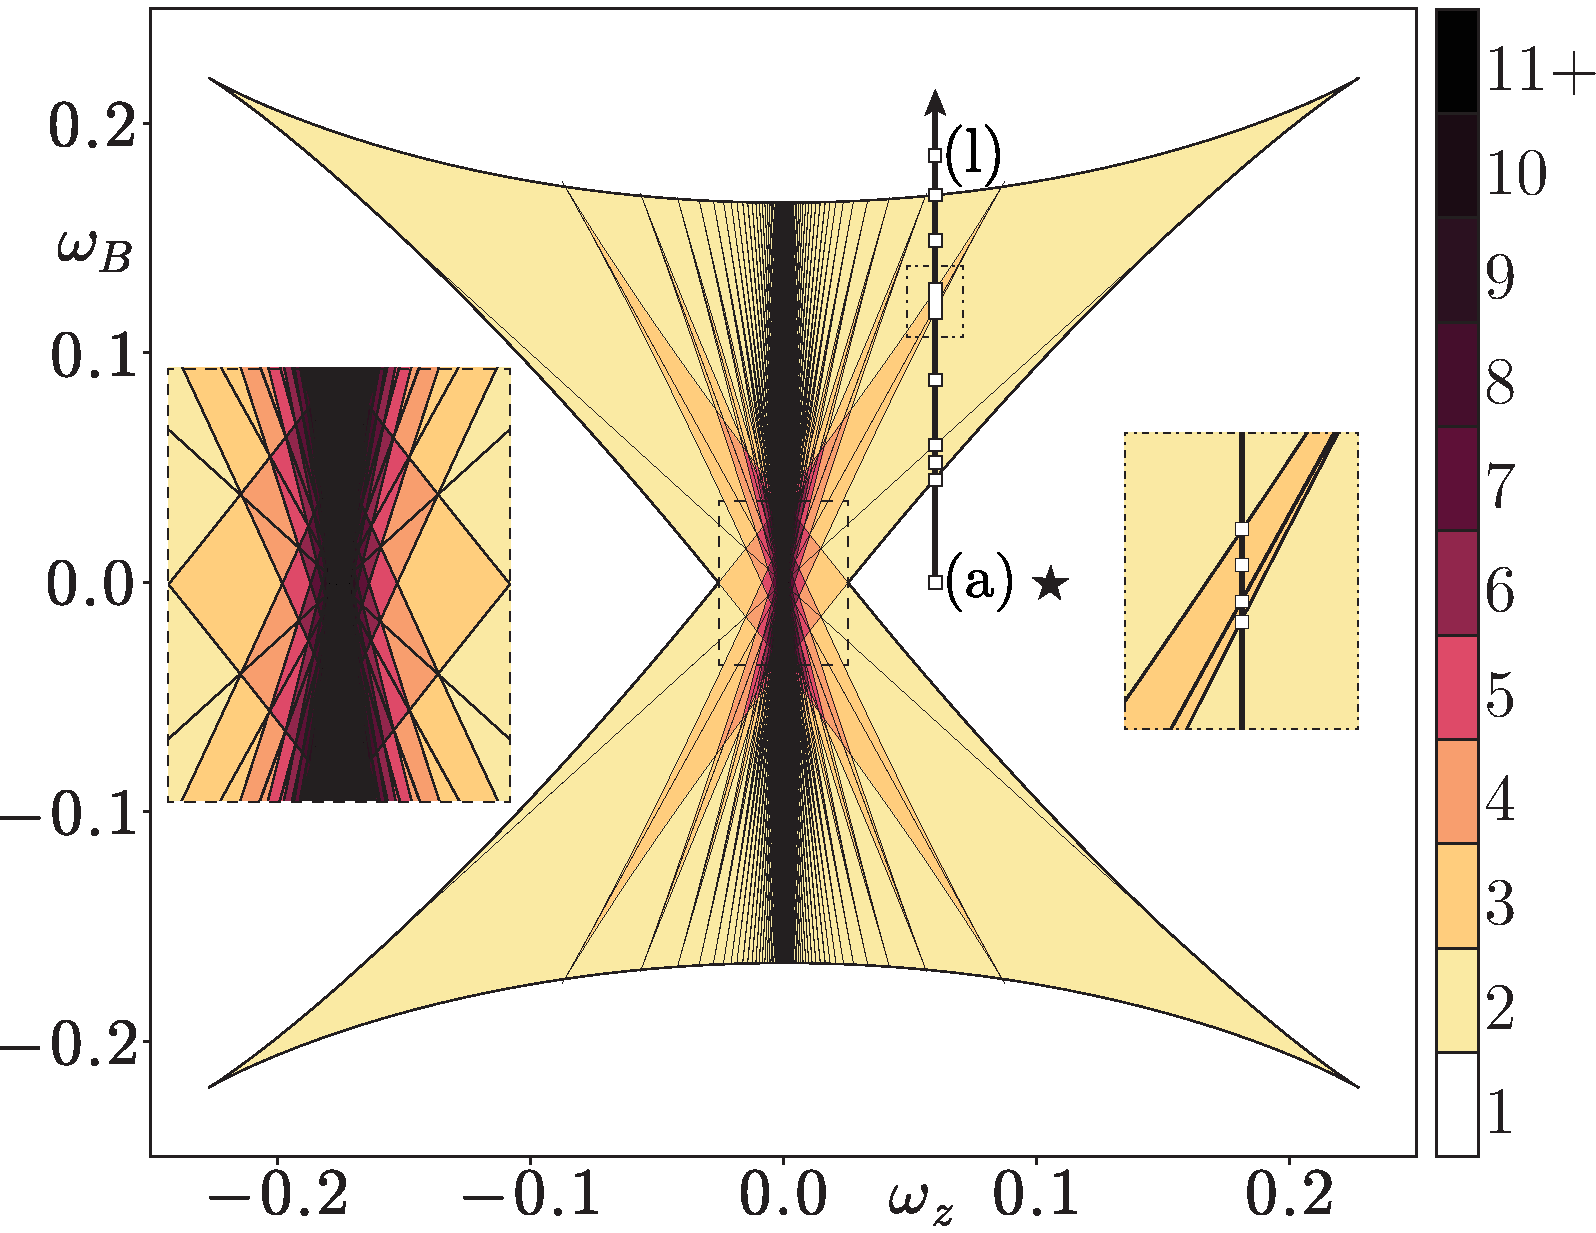
\includegraphics[width=\linewidth]{Images/EGM_components_2D_coloured_with_closeup.pdf}

    \caption{Regions in the $(\wz, \wB)$-plane indicating the number of isolated EGM-components exist up to 11 according to the colourbar. 
    A closeup of the region with the highest density of EGM components is shown in the inset.
    The values of $(\wz,\wB)$ plotted in Figure~\ref{fig:EGM_fold_varywB} are indicated by the dots along the line $\wz=0.06$.}

    \label{fig:EGM_components}
\end{figure}
%
\begin{figure}[!t]
    \centering
    \begin{overpic}[width=\linewidth]{Images/EGM_fold_varywB_wz006.pdf}
        % Row a
        \put(11.5,96){(a)}
        \put(36.5,96){(e)}
        \put(61.2,96){(i)}
        % Row b
        \put(11.5,72){(b)}
        \put(36.5,72){(f)}
        \put(61.2,72){(j)}
        % Row c
        \put(11.5,48){(c)}
        \put(36.5,48){(g)}
        \put(61.2,48){(k)}
        % Row d
        \put(11.5,24.5){(d)}
        \put(36.5,24.5){(h)}
        \put(61.2,24.5){(l)}
    \end{overpic}

    \caption{Graph of the EGM component function $G(\w_s)$ from \eqref{eq:EGM_components} for $\wz = 0.06$ and varying $\wB$, whose particular values are indicated by dots along the line $\wz=0.06$ in Figure~\ref{fig:EGM_components}.
    The roots (hollow circles) bound intervals of $\w_s$ values corresponding to egm components (thick lines); one interval always contains $\w_s = 0$ (the free running laser mode) and another contains the grating's Bragg frequency for $\wB \in [0.04505, 0.16895]$.
    }

    \label{fig:EGM_fold_varywB}
\end{figure}
%
The advantages of the discretised model in understanding the mode structure become apparent when examining the bifurcation patterns of the EGM solutions.
Analytic expressions for the EGM components and their bifurcation points can be derived from the discretised model, providing valuable insights into the stability and dynamics of the system.
The number of EGM components can be studied by setting the envelope of $f(\w_s)$ given by \eqref{eq:discretised_ws_envelope} equal to $g(\w_s)$, which yields the $\w_s$ values at the intersections as the roots of the function
%
\begin{equation}
    \label{eq:EGM_components}
    G(\w_s) = \w_s^2 - (1+\a^2)\left( \eta \, (1-t) \frac{S_N}{S} \right)^2.
 \end{equation}
 %
Moreover, these roots bound intervals of $\w_s$-values that correspond to different EGM-components, so that the function $G(\w_s)$ presents a geometrical interpretation of the EGM-components. 
The number of EGM-components changes when fold points (with respect to $\w_s$) of the envelope pass through the line $g(\w_s)$. 
These fold points are given by roots of the first derivative of \eqref{eq:EGM_components} with respect to $\w_s$, that is, by
%
\begin{gather}
    \label{eq:EGM_components_fold}
    \begin{aligned}
        \frac{\partial G}{\partial \w_s} &= \dt (1+\a^2)\left( \eta \, (1-t) \frac{S_N}{S} \right)^2 \times \\ 
        &\bigg(  \frac{t}{S^2} \sin(\phi_\text{F}) - N \frac{t^{N}}{{S_N}^2}\sin(N\phi_\text{F}) \bigg) + \w_s = 0.
    \end{aligned}
\end{gather}
%
\par
%
The locus of the passage through folds as the FBG parameters $\wz$ and $\wB$ are varied can be found with the pseudo-arclength continuation routines of \texttt{DDE-BifTool} \cite{sieber2014dde} to simultaneously solve the implicit equations \eqref{eq:EGM_components} and \eqref{eq:EGM_components_fold}, that is, by solving $G(\w_s) = \sfrac{dG}{d\w_s} = 0$.
Figure~\ref{fig:EGM_components} shows the locus of the passage through folds (computed by continuation) in projection onto the $(\w_s, \wB)$-plane.
In the white region outside the curve shown in Figure~\ref{fig:EGM_components} one finds a single EGM-component, while inside the shaded region there are two or more isolated EGM-components.
The outermost curves meet at cusp points.
Within this region containing more than one isolated component, further bifurcations can occur as $\wz$ and $\wB$ vary allowing for the emergence of an arbitrariry number of EGM components, as illustrated by the inset of Figure~\ref{fig:EGM_components}.
An explicit example of this behaviour can be seen in Figure~\ref{fig:EGM_fold_varywB}(a)-(l) which shows the the transition


the graph of $G(\w_s)$ for $\wz = 0.06$ and increasing $\wB \in [0, 0.018]$.
The number of EGM-components changes when fold points (with respect to $\w_s$) of the envelope pass through the line $G(\w_s) = 0$.
Finally, we note that the region shown in Figure~\ref{fig:EGM_components} scales linearly with the effective feedback strength $\eta (1-t) \sqrt{1 + \alpha^2}$.
In other words, the region retains its shape yet grows linearly with $\eta (1-t) \sqrt{1 + \alpha^2}$.
%
\par
%

%
\subsection{Stability Fluctuations}
\label{subsec:lichaos_skenderas}
%
\begin{figure}[t]
    
    \begin{overpic}[width=0.9\linewidth]{Images/Reflection_zero_overlap.pdf}
        \put(2,86){(a)}
        \put(2,43){(b)}
    \end{overpic}

    \caption{Caption}
    
    \label{fig:zero_overlap}
\end{figure}
%
It is important to note that while the locations of zeros in the discretised model are uniform, is only the case for FBGs which have relatively low reflectivities, see Figure~\ref{fig:uniform_spectra_varykL}. 
For this, re 
%

\begin{figure}[t]
    \flushleft
    \begin{overpic}[width=0.845\linewidth]{Images/Li_chaos_heatmap_image.pdf}
        \put(-2,77){(a)}
    \end{overpic}\\
    \vspace{-0.5em}
    \begin{overpic}[width=0.99\linewidth]{Images/discretised_Lichoatic_wBeta_comparison_hopfs_minbifs_ai.pdf}
        \put(-2,65){(b)}
    \end{overpic}\\
    \vspace{-0.5em}
    \begin{overpic}[width=\linewidth]{Images/discretised_Lichoatic_wBeta_comparison_lyapunovs.pdf}
        \put(-2,70){(c)}
    \end{overpic}

    \caption{Comparison between two parameter dynamical mappings of output intensity for a convolved FBG feedback form of $F(t)$ \cite{li2012distributed,li2015chaotic,li2020stable} (a) 
    and the discretised FBG feedback form of $F(t)$ in the parameter space of feedback strength ($\xi_f$ in (a) and equivalent $\eta$ in (b)) 
    and grating detuning frequency ($\Delta f$). 
    In (a), the laser output intensity is stable (white), period-one oscillatory (red), quasi-periodic pulsating (gray), period-doubled oscillatory (yellow), and chaotic (black). 
    In (b), the laser output is in steady-state (white), period-one oscillatory (red), period-two (yellow), and period 3 to very large period in a gradient from grey to black. 
    In (c) parameter sweeps are performed in all four directions, with Hopf bifurcations of steady state EGMs overlayed.}
    
    \label{fig:Li_chaos}
\end{figure}
%
\par
%
Finally, we compare our model to the most recent work on semiconductor lasers under FBG feedback by \Skenderas \textit{ et al.} \cite{skenderas2021feedback,skenderas2024impact}. 
In contrast to the previous two models, where nondimensionalisations and approximations were required before direct comparisons could be made, the form of the equations analysed mirror the equations presented in this work, 
using parameter values $(\a, P, T, \tau) = (3, 1, 1000, 1000)$, except for the use of a convolution feedback term $F(t)$ of the form \eqref{eq:convolution}. 
The results presented by \Skenderas \textit{ et al.} therefore serve as the most suitable basis for comparisons in the accuracy of the derived discretised model. 
Given the complexity of analysing the LK equations under FBG feedback using a convolution term, the results presented, 
like those previously studied, are obtained solely through analysis of time series obtained through numerical integration. 
The main focus of their analysis is in characterising the interplay between the lasers relaxation oscillations (ROs) and the FBG reflection zeros as a function of feedback rate $\eta$ and grating bandwidth $\wz$ for varying feedback phase $C_p$ and grating detuning $\omega_B$. 
%
\par
%
ROs are the most typical type of oscillation that one would expect in semiconductor lasers. 
They are damped intensity fluctuations that occur when the laser transitions between steady states, typically after a sudden change in injection current, 
and arise from the dynamic interplay between photon density and carrier density in the laser cavity. 
When the carrier population is perturbed, it overshoots the steady-state value, causing oscillations in output power at a characteristic frequency known as the relaxation oscillation frequency $\w_\text{RO}=\sqrt{2P/T}$, 
which form the dominant side lobes either side of the centre frequency in the Fourier spectrum of a semiconductor laser. 
Exciting the ROs of a laser can lead to a more unstable laser, and therefore one would expect that lower amount of feedback would cause the laser to transition from steady output to oscillatory and then more unstable outputs. 
%
\par
%
The strategy employed by the authors to observe this behaviour is by tracking the Hopf bifurcation of the steady state of the laser in the $(L_\text{FBG},\eta)$-plane, 
where the grating length $L_\text{FBG}$ can be used to control the grating bandwidth $\wz$ as discussed in \ref{sec:EGM_discretised}. 
As discussed in \ref{sec:FBG}, varying the grating length also changes the grating reflectivity, therefore, when using this model, grating parameters must be simultaneously varied to solely vary its bandwidth. 
This is not an issue with the discretised reflections model as bandwidth $\wz$ and thus length $L_\text{FBG}$ can be varied independent of reflectivity using \ref{eq:wz_approx}
%
\begin{equation}
    L [\text{m}] \approx \frac{\pi c \tau_p}{\wz \neff} 
\end{equation}
%
where $\tau_p$ is the photon lifetime used to rescale time in this form of the LK equations as discussed in Section~\ref{sec:EGM_discretised}.
%
\par
%
\begin{figure}[!t]
    \flushright
    \begin{overpic}[width=\linewidth]{Images/discretised_Skenderas_wzeta_Cpcomparison_N20.pdf}
        \put(-3,55){(a)}
    \end{overpic}\\
    \hspace{-0.5em}
    \begin{overpic}[width=0.98\linewidth]{Images/discretised_Skenderas_wBeta_image.pdf}
        \put(-3,75){(b)}
    \end{overpic}\\
    \hspace{-0.5em}
    \begin{overpic}[width=0.97\linewidth]{Images/discretised_Skenderas_wBeta_comparison_minbifs_ai.pdf}
        \put(-3,75){(c)}
    \end{overpic}

    \caption{The evolution of Hopf bifurcation tracking the stability fluctuations as a function of $L_\text{FBG}$ at zero detuning for different values of the feedback offset phase $C_p$ equal to 
    $0$ (blue), $\pi /4$ (yellow), $\pi/2$ (violet), $2\pi/3$ (green), $\pi$ (cyan), $3\pi/2$ (maroon), and $7\pi/4$ (orange). Comparison between two parameter dynamical mappings of output intensity for a convolved FBG feedback form of $F(t)$ \cite{li2012distributed,li2015chaotic,li2020stable} (a) 
    and the discretised FBG feedback form of $F(t)$ in the parameter space of feedback strength ($\xi_f$ in (a) and equivalent $\eta$ in (b)) and grating detuning frequency ($\Delta f$). 
    In (a), the laser output intensity is stable (white), period-one oscillatory (red), quasi-periodic pulsating (gray), period-doubled oscillatory (yellow), and chaotic (black). 
    In (b), the laser output is in steady-state (white), period-one oscillatory (red), period-two (yellow), and period 3 to very large period in a gradient from grey to black. 
    In (c) parameter sweeps are performed in all four directions, with Hopf bifurcations of steady state EGMs overlayed}
    
    \label{fig:Skenderas_wBeta}
\end{figure}
%

